% !Mode:: "TeX:UTF-8"
% !TEX root = tjumain.tex

\iffalse
\bibliography{reference/reference.bib} % 欺骗latextools获取bib文件
\fi

%%%%%%% 正文 %%%%%%%

\chapter{引言}

笔者在学习高中数学时,无意间接触到了Taylor公式.对于这样一个可以用来逼近函数值的定理,笔者好奇其是否能在物理学中有所应用,于是在预习物理时特意留心,注意到了两个可以直接利用Taylor公式(方法)证明的命题,以及若干利用等价无穷小解决的问题.本文简要记录了这些结论.

由于笔者并没有专门研究物理学,本文中的纰漏在所难免,特此致歉.

\chapter{Taylor公式及其证明}

\begin{theorem}{\textbf{带Peano余项的Taylor公式}\cite{ayumu}}
	设函数$f(x)$在$x_0$处有$n$阶导数,则当$x \to x_0$时,$$f(x) = f(x_0) + \frac{1}{1!}f'(x_0)(x-x_0) + \frac{1}{2!}f''(x_0)(x-x_0)^2 + \cdots + \frac{1}{n!}f^{(n)}(x_0)(x-x_0)^n + o[(x-x_0)^n]$$
\end{theorem}
\begin{proof}
	对$n$进行归纳证明:记$$T_{n}(f,x_0;x):=f(x_0) + \frac{1}{1!}f'(x_0)(x-x_0) + \frac{1}{2!}f''(x_0)(x-x_0)^2 + \cdots + \frac{1}{n!}f^{(n)}(x_0)(x-x_0)^n$$
	当$n=1$时,命题即为$$f(x)=f(x_0)+f'(x_0)(x-x_0)+o(x-x_0),~x \to x_0$$
	由无穷小增量公式,该命题成立; \\
	假设当$n=k$时命题成立.由于
	$$T_{k+1}(f,x_0;x)=f(x_0) + \frac{1}{1!}f'(x_0)(x-x_0) + \frac{1}{2!}f''(x_0)(x-x_0)^2 + \cdots + \frac{1}{(k+1)!}f^{(k+1)}(x_0)(x-x_0)^{k+1}$$
	故
	$$T'_{k+1}(f,x_0;x)=f'(x_0) + \frac{1}{1!}f''(x_0)(x-x_0) + \cdots + \frac{1}{k!}f^{(k+1)}(x_0)(x-x_0)^{k} = T_k(f',x_0;x)$$
	由l’Hôpital法则和归纳假设可知$$\lim_{x \to x_0} \frac{f(x)-T_{k+1}(f,x_0;x)}{(x-x_0)^{k+1}} = \frac{1}{k+1} \lim_{x \to x_0} \frac{f'(x)-T_{k}(f',x_0;x)}{(x-x_0)^{k}} = 0$$
	由归纳原理知原命题成立.
\end{proof}

可以认为,Taylor公式通过一个函数在某点附近的信息来估计函数值.更确切地说,它通过一个多项式拟合原函数.

在应用Taylor公式时,我们倾向于尽可能多地简化该式子.令$x_0=0$,即得到\textbf{Maclaurin公式}.

\begin{corollary}{\textbf{Maclaurin公式}}
	设函数$f(x)$在$0$处有$n$阶导数,则当$x \to 0$时,$$f(x)=f(0)+\frac{f'(0)}{1!}x + \frac{f''(0)}{2!}x^2 + \cdots + \frac{f^{(n)}(0)}{n!}x^n + o(x^n)$$
\end{corollary}

微元法中应用的“等价无穷小”本质上就是Maclaurin公式.因而在后文主要讨论的都是该公式的应用.


\chapter{Taylor公式(方法)在物理学中的直接应用}

\section{推导变速直线运动公式}

先来看一个简单的结论.在匀变速直线运动中,位移关于时间的函数$x(t)$满足$$x(t) = x_0 + v_0t + \frac{1}{2}at^2$$
我们好奇能否将这个形式进行推广?如果知道物体在$0$时刻处的速度、加速度、加速度的变化率、加速度的变化率的变化率$\cdots$能否给出$x(t)$的表达式?

注意到,上式与Maclaurin公式的形式很像.若设$x(t)$表示在直线运动中从$0$时刻到$t$时刻中物体的位移量,这意味着$$x(t) = x(0) + \frac{1}{1!} x'(0)t + \frac{1}{2!} x''(0)t^2$$
然而这个形式不完全等价于Maclaurin公式,因为该公式的效用极限过程是$t \to 0$.换个思路,我们可以用接近于Taylor公式证明的方法来证明该加强命题:

\begin{proposition}{}
	设$a_i~(i=0,1,2,\cdots)$为常数,在$x(t)$的某一阶导函数为常值函数时,有$$x(t) = \sum_{i=0}^{\infty} a_ix^{(i)}(0) t^{i} = a_0x(0) + a_1x'(0)t + a_2x''(0)t^2 + \cdots$$
	其中$\{ a_n \}_{n=0}^{\infty}$满足$a_n = \dfrac{1}{n!}$.
\end{proposition}
\begin{remark}
	该命题的形式与Legendre定理类似.因为对任意$n>N$都有$x^{(n)}(0)=0$,故这是个有限项多项式.
\end{remark}
\begin{remark}
	若$x(t)$不存在任一阶导函数为常值函数,可以取某个足够大的$n$来近似计算.
\end{remark}
\begin{proof}
	设$x(t)$的第$n$阶导函数为常值函数,对$n$进行归纳证明.记$$T_n(x;t) := x(t) = x(0) + \frac{1}{1!} x'(0)t + \frac{1}{2!} x''(0)t^2 + \cdots + \frac{1}{n!} x^{(n)}(0)t^n$$
	$1^{\circ}~$当$n=1$时,由于此时物体作匀速直线运动,$x(t)=x(0)+x'(0)t$自然成立. \\
	$2^{\circ}~$假设$n=k$时命题成立.在$n=k+1$时,由于
	$$T_{k+1}(x;t) = x(0) + \frac{1}{1!} x'(0)t + \frac{1}{2!} x''(0)t^2 + \cdots + \frac{1}{(k+1)!} x^{(k+1)}(0)t^{k+1}$$
	$$T'_{k+1}(x;t) = x'(0) + \frac{1}{1!} x''(0)t + \frac{1}{2!} x'''(0)t^2 + \cdots + \frac{1}{k!} x^{(k+1)}(0)t^k = T_{k}(x';t)$$
	由归纳假设,$T_k(x',t)=x(t)$.故$x(t)=T_{k+1}(x;t)$. \\
	由数学归纳原理可知命题成立.
\end{proof}

命题3.1提供了一个有趣的直觉:如果能搞清楚某物体任一时间下的运动状态,我们就能推导它的运动全程.这个直觉被应用在了刘慈欣的科幻小说《镜子》\cite{liucixin}中:文中气象模拟员白冰通过对宇宙大爆炸时有限个物理量的控制模拟出了我们的宇宙.不过显然对于一个混沌系统不能这么搞.

\section{推导近地重力势能公式}

上一小节似乎是杀鸡用了牛刀.本小节更能体现出Taylor公式在处理近似时的重要作用.

\begin{proposition}
	在选取地表为零势能点时,近地物体的重力势能为$$E_{PG} \approx mgh$$
\end{proposition}
\begin{remark}
	当物体的质量到达天文质量级时,这个估计将会极不准确,因而只讨论物体质量远小于地球质量的情况.
\end{remark}

对于一个近地物体,设地球半径$R$,地表与该物体距离$h$,地球、该物体质量分别为$M,m$,$G$为万有引力常数,选择无穷远处为势能零点,则该物体的引力势能为(将其看做关于$h$的函数)$$E_P(h) = - \frac{GMm}{R+h}$$
由于$h \ll R$,令$h \to 0$,由Maclaurin公式,此时有
\begin{align*}
	E_P(h) &= E_P(0)+\frac{E'_P(0)}{1!}h + o(h^2) \\
	&\approx -\frac{GMm}{R} + \frac{GMm}{R^2} h
\end{align*}
由黄金代换公式,$$E_P(h) \approx -\frac{GMm}{R} + mgh$$
注意到这个式子的势能零点是无穷远处,而近地重力势能的势能零点是地表.这两个零势能点的势能差值等于地表处因(近似等价于)球心的万有引力而具有的势能(此时零势能点为无穷远处),这个值恰好为$$-\frac{GMm}{R}$$
于是近地处物体重力势能为(零势能点为地表)$$E_{PG} \approx mgh$$

\chapter{等价无穷小的应用}

由Maclaurin公式,可以得到以下重要的等价无穷小:

\begin{proposition}
	当$x \to 0$时, 
	$$(1+x)^{\alpha} -1 \sim \alpha x, \qquad \sin x \sim x \sim\tan x, \qquad 1-\cos x \sim \dfrac{x^2}{2}$$
\end{proposition}

这些结论是显而易见的.



\begin{example}
	如图i所示,岸上一小人以恒定速度$v$拉动绳子的一头,船上的小人抓住绳子的另一头,求船速$v'$.
	
	\begin{center}
		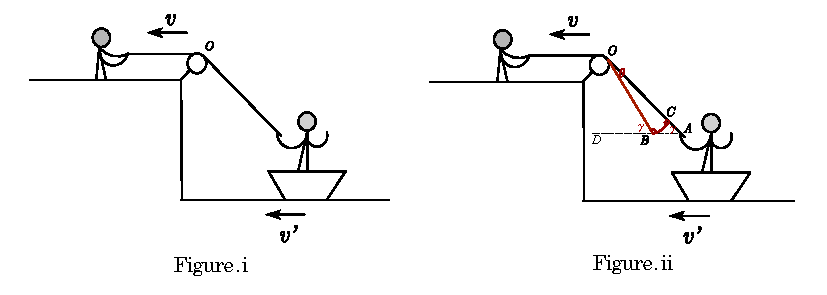
\includegraphics[width=14cm]{4.1.pdf}
	\end{center}
\end{example}
\begin{solution}
	如图ii所示,在一段极短的时间$\Delta t$内,设绳子的一头从$A$移动到$B$,过点$B$作$BC \bot OB$. \\
	在$\vartriangle OBC$中,由于$\tan \theta \sim \sin \theta$,又$BC = \tan \theta OB = \sin \theta OC$,故可看做$OC=OB=l$,此时$\angle OBC = 90^{\circ}$.同理可知$\angle OCB = 90^{\circ}$.于是$\overset{\LARGE{\frown}}{BC} = \theta l = \tan \theta l = BC$,可将$\overset{\LARGE{\frown}}{BC}$看做直线. \\
	考虑$\angle OBD=\gamma$,于是$\angle CBA=90^{\circ} - \gamma$,那么$\angle CAB = \gamma$.在直角三角形$\vartriangle ABC$中,$AB = v' \Delta t$,$AC = v \Delta t$,故$v \Delta t = \cos \gamma v' \Delta t$,解得$v' = \dfrac{v}{\cos \gamma}$.
\end{solution}





%%%%%%% 结论 %%%%%%%

\addcontentsline{toc}{chapter}{结\quad 论} %添加到目录中

\chapter*{结\quad 论}

逸一时,误一世。逸久逸久,罢已龄!
